\documentclass[12pt, preprint]{aastex}
%\documentclass[12pt, preprint]{emulateapj}
\usepackage[breaklinks,colorlinks, 
urlcolor=blue,citecolor=blue,linkcolor=blue]{hyperref}
\usepackage{graphicx}	% For figures
\usepackage{natbib}	% For citep and citep
\usepackage{amsmath}	% for \iint
\usepackage{mathtools}
\usepackage{bm}
\usepackage[breaklinks]{hyperref}	% for blackboard bold numbers
\usepackage{hyperref}
\usepackage{algorithmic,algorithm}
\hypersetup{colorlinks}
\usepackage{color}
\usepackage{morefloats}
\definecolor{darkred}{rgb}{0.5,0,0}
\definecolor{darkgreen}{rgb}{0,0.5,0}
\definecolor{darkblue}{rgb}{0,0,0.5}
\hypersetup{ colorlinks,
linkcolor=darkblue,
filecolor=darkgreen,
urlcolor=darkred,
citecolor=darkblue}

\DeclareMathOperator*{\argmax}{arg\,max}
\newcommand{\beq}{\begin{equation}}
\newcommand{\eeq}{\end{equation}}
\newcommand{\lang}{\langle}
\newcommand{\ra}{\rangle}
\newcommand{\vep}{\bm{\epsilon}}
\newcommand{\ep}{\epsilon}
\newcommand{\pars}{\vec{\theta}}
\newcommand{\dev}{\mathrm{d}}
\newcommand{\ngal}{n_{g}}
\newcommand{\gmf}{g(N)}
\newcommand{\mr}{M_{\rm r}}
\newcommand{\rpp}{r_{\rm p}}
\newcommand{\mzero}{\log M_{0}}
\newcommand{\mone}{\log M_{1}}
\newcommand{\mmin}{\log M_{\rm min}}
\newcommand{\sigmam}{\sigma_{\log \rm M}} 
\newcommand{\wpp}{w_{\rm p}} 

\newcommand{\acen}{\mathcal{A}_{\rm cen}}
\newcommand{\asat}{\mathcal{A}_{\rm sat}}
%\newcommand{\comment}[1]{{\bf \textcolor{red}{ #1}}}
\newcommand{\todo}[1]{{\em \textcolor{red}{ #1}}}

%% preprint2 produces a double-column, single-spaced document:

%% \documentclass[preprint2]{aastex}

%% Sometimes a paper's abstract is too long to fit on the
%% title page in preprint2 mode. When that is the case,
%% use the longabstract style option.

%% \documentclass[preprint2,longabstract]{aastex}

%% If you want to create your own macros, you can do so
%% using \newcommand. Your macros should appear before
%% the \begin{document} command.
%%
%% If you are submitting to a journal that translates manuscripts
%% into SGML, you need to follow certain guidelines when preparing
%% your macros. See the AASTeX v5.x Author Guide
%% for information.


%% You can insert a short comment on the title page using the command below.

%\slugcomment{Not to appear in Nonlearned J., 45.}

%% If you wish, you may supply running head information, although
%% this information may be modified by the editorial offices.
%% The left head contains a list of authors,
%% usually a maximum of three (otherwise use et al.).  The right
%% head is a modified title of up to roughly 44 characters.
%% Running heads will not print in the manuscript style.

%\shorttitle{Collapsed Cores in Globular Clusters}
%\shortauthors{Djorgovski et al.}

%% This is the end of the preamble.  Indicate the beginning of the
%% paper itself with \begin{document}.

\begin{document}

%% LaTeX will automatically break titles if they run longer than
%% one line. However, you may use \\ to force a line break if
%% you desire.
\title{Inference of probability distributions over redshifts and other galaxy properties}

\author{A.I. Malz\altaffilmark{1}}
\author{Mohammadjavad Vakili\altaffilmark{1}}
\author{Michael Schneider\altaffilmark{2}}
\author{Jeffrey Newman\altaffilmark{3}}
\altaffiltext{1}{Center for Cosmology and Particle Physics, Department of Physics,
  New York University, 4 Washington Pl., room 424, New York, NY 10003, USA}
\altaffiltext{2}{LLNL}
\altaffiltext{3}{U.Pitt.}
%%\title{Collapsed Cores in Globular Clusters, \\
%%    Gauge-Boson Couplings, and AAS\TeX\ Examples}

%% Use \author, \affil, and the \and command to format
%% author and affiliation information.
%% Note that \email has replaced the old \authoremail command
%% from AASTeX v4.0. You can use \email to mark an email address
%% anywhere in the paper, not just in the front matter.
%% As in the title, use \\ to force line breaks.


\begin{abstract}
Posterior probability distributions over photometric redshift (photo-$z$) are rapidly replacing photo-$z$ point estimators as data products of current and future galaxy surveys.  It is desirable not only to have probabilities over redshift $z$ but also over other parameters $\vec{\alpha}$, both directly measurable (ellipticity, size, etc.) and not (stellar mass, star formation history, etc.).  Such hypothetical data products could be informative for studies of weak gravitational lensing, large-scale structure, and supernova cosmology if approached from a hierarchical Bayesian perspective.  This work studies $p(z,\vec{\alpha})$ data products from two perspectives.  We apply various methods for deriving posterior probability distributions over $z$ and $\vec{\alpha}$.  We also explore usage cases for these data products and propose approaches to inference based upon them.
\end{abstract}

\section{Introduction}

\begin{figure}
\includegraphics[width=0.5\textwidth]{../fig/1pt.png}
\caption{This figure shows a graphical model for the problem we wish to investigate.  The photometric data $\vec{d}$ is completely characterized by the redshift $z$ and the parameters $\vec{\alpha}$ that determine the template shape.  $z$ and $\alpha$ are drawn from a distribution function specified by parameters comprising $\vec{\Phi}$.}
\label{fig:1pt}
\end{figure}

\section{Data}

We use the Buzzard mock galaxy catalog for this work because it employs a generative model by which data is consistently produced by physically-motivated processes.

\section{Methods}

We attempted to derive $p(z,\vec{\alpha})$ data products using methods from two broad classes, machine learning and template fitting.

\subsection{Machine Learning}

One weakness of machine learning is that it cannot extrapolate, so if the training set does not span the full space of the test set, the results will be unreliable.

\subsubsection{k Nearest Neighbors}

\subsection{Random Forests}

\subsection{Template Fitting}

\section{Results}

\subsection{Machine Learning}

The machine learning methods are sensitive to the size and diversity of the training set.

\subsubsection{k Nearest Neighbors}

The nearest neighbor algorithm produces results using the least resources and is insensitive to the number of classes.

\begin{figure}
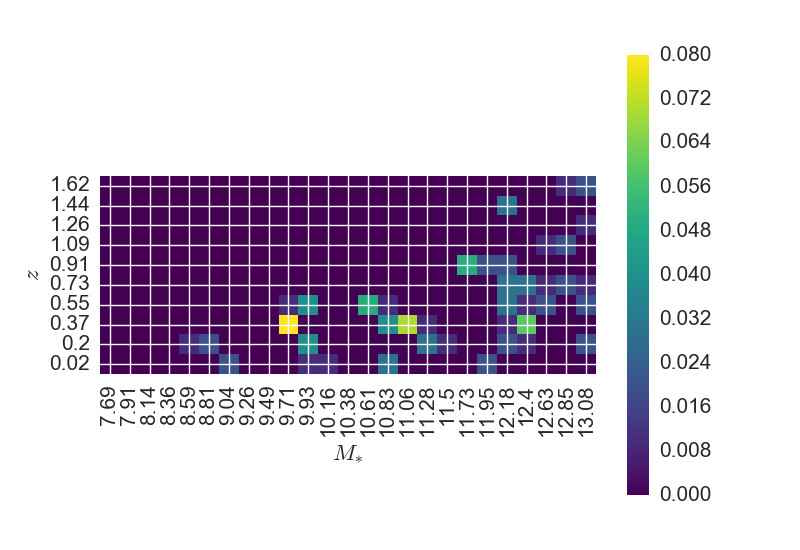
\includegraphics[width=1.\textwidth]{../fig/knn3.png}\\
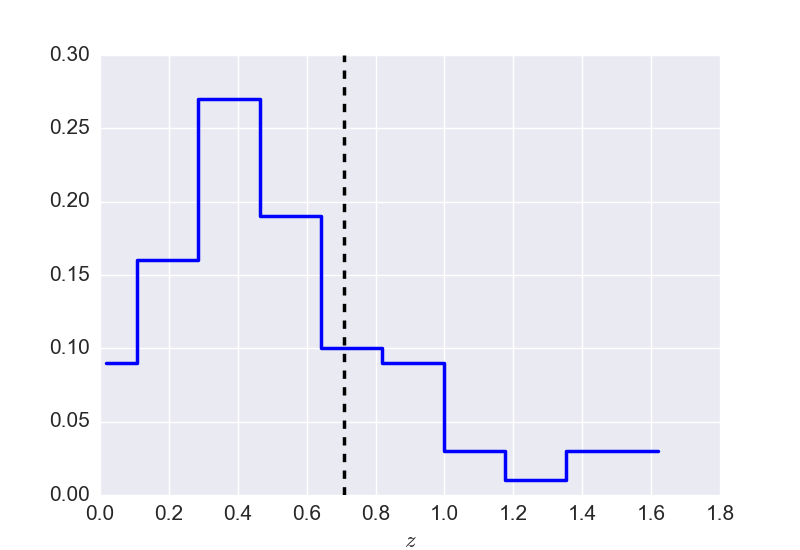
\includegraphics[width=0.5\textwidth]{../fig/knn3z.png}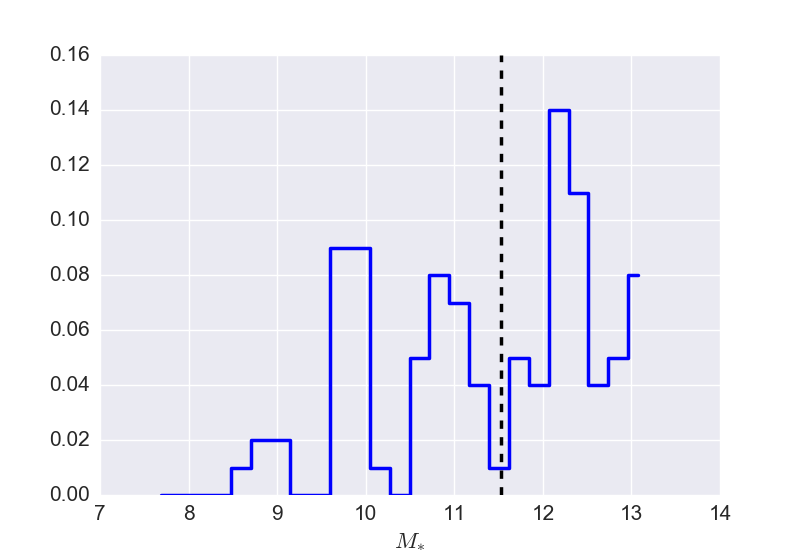
\includegraphics[width=0.5\textwidth]{../fig/knn3m.png}
\caption{}
\label{fig:knn-bad}
\end{figure}

\begin{figure}
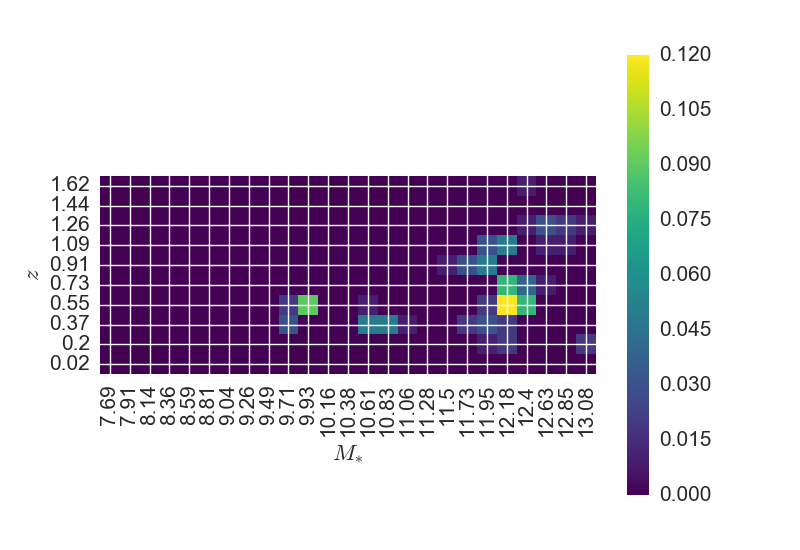
\includegraphics[width=1.\textwidth]{../fig/knn8.png}\\
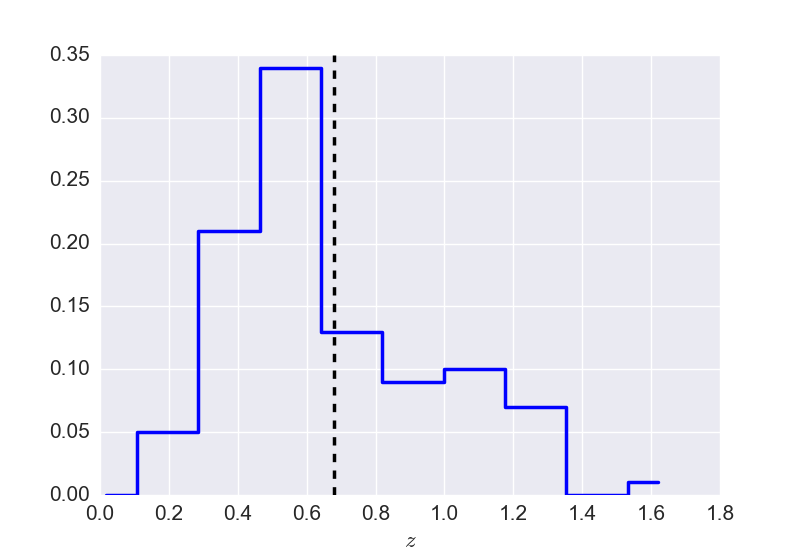
\includegraphics[width=0.5\textwidth]{../fig/knn8z.png}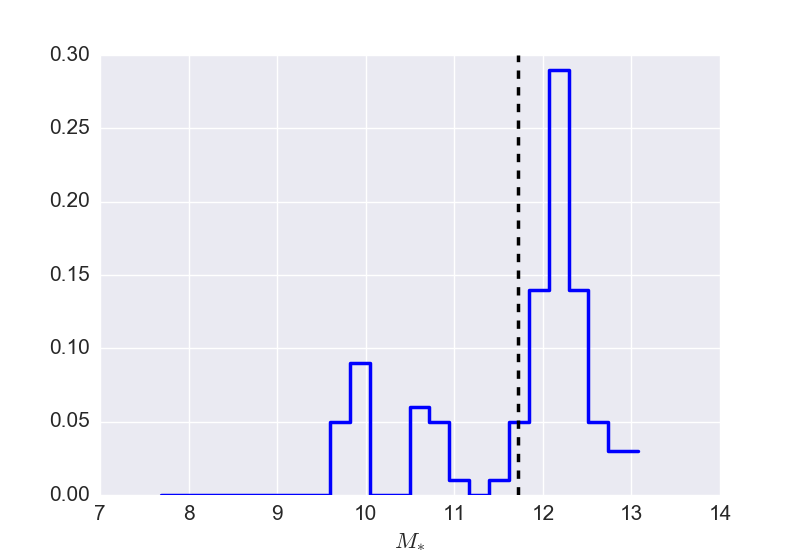
\includegraphics[width=0.5\textwidth]{../fig/knn8m.png}
\caption{}
\label{fig:knn-good}
\end{figure}

\subsection{Random Forests}

Random forests is sensitive to the number of classes and is very memory intensive.

\begin{figure}
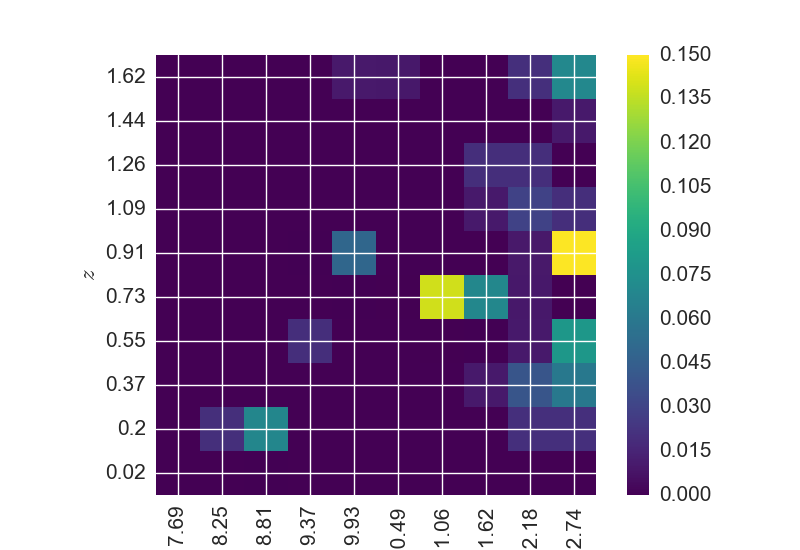
\includegraphics[width=0.3\textwidth]{../fig/rf3.png}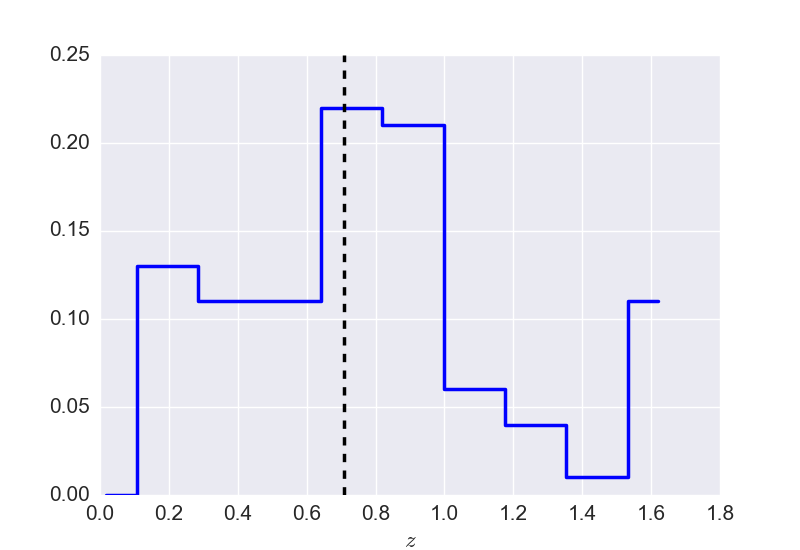
\includegraphics[width=0.3\textwidth]{../fig/rf3z.png}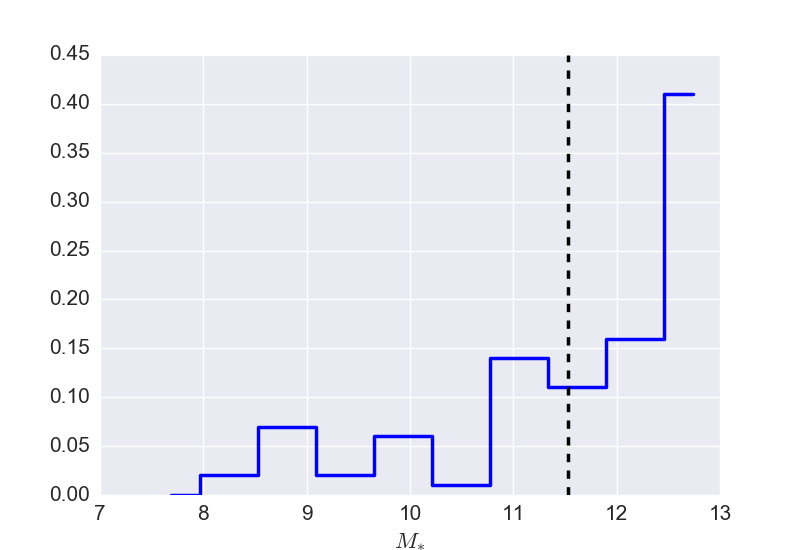
\includegraphics[width=0.3\textwidth]{../fig/rf3m.png}
\caption{}
\label{fig:rf-good}
\end{figure}

\begin{figure}
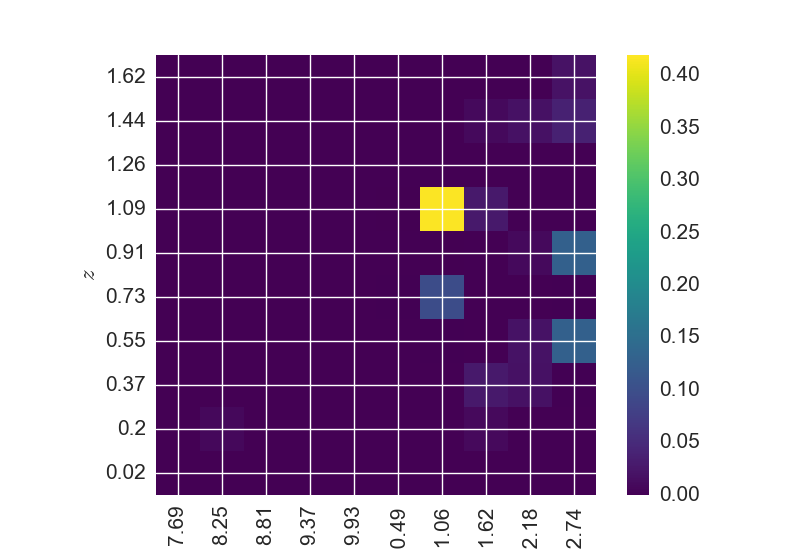
\includegraphics[width=0.3\textwidth]{../fig/rf8.png}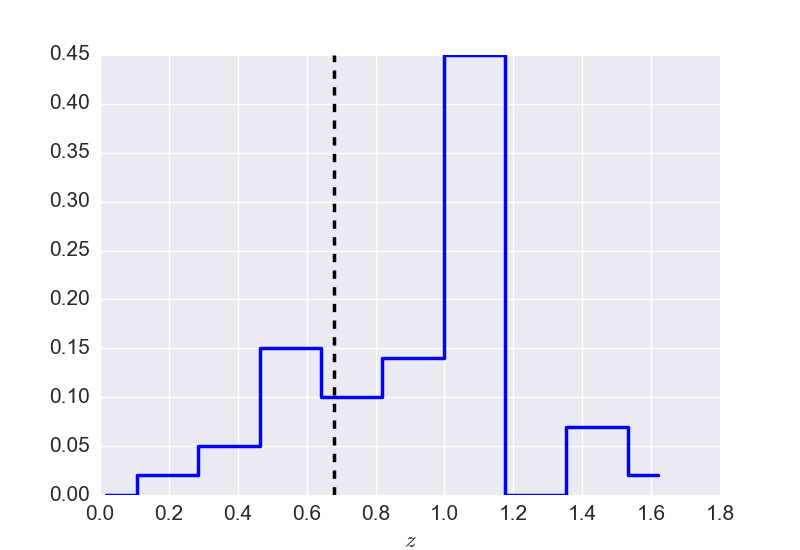
\includegraphics[width=0.3\textwidth]{../fig/rf8z.png}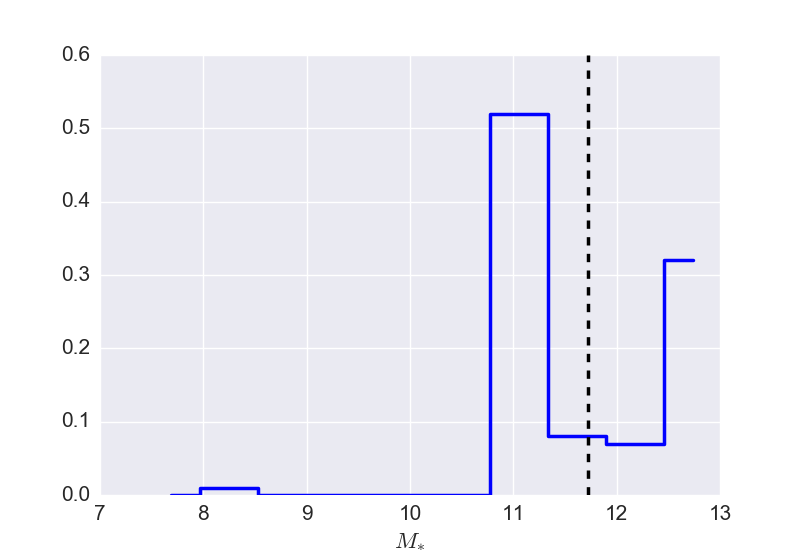
\includegraphics[width=0.3\textwidth]{../fig/rf8m.png}
\caption{}
\label{fig:rf-good}
\end{figure}

\subsection{Template Fitting}

Template fitting with MCMC is much slower and must be run on individual galaxies in the test set.  Rather than fitting $\alpha$, it fits for the template coefficients, which may then be backtracked to $\alpha$.

\begin{figure}
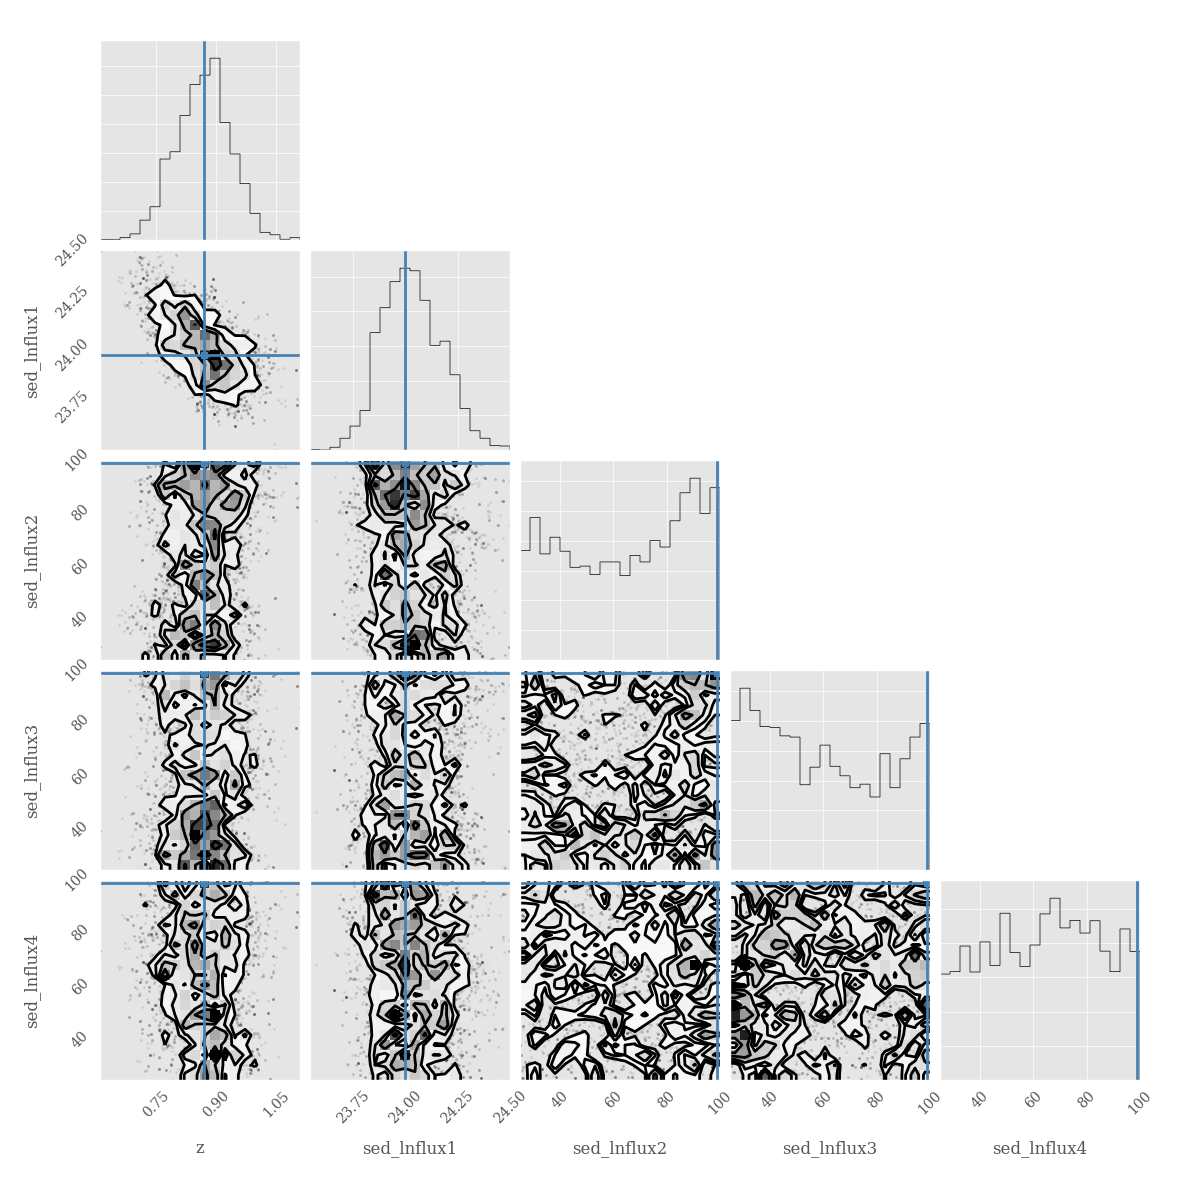
\includegraphics[width=1.\textwidth]{../fig/sed_model_galsim_corner.png}
\caption{}
\label{fig:temp}
\end{figure}

\section{Discussion}

\section{Conclusion}

\end{document}

%%
%% End of file `sample.tex'.
%% End of file `sample.tex'.
